% One-slide, editable Beamer + TikZ template. Compile with pdflatex.
\documentclass[aspectratio=169,10pt]{beamer}
\usepackage[T1]{fontenc}
\usepackage{lmodern}
\usepackage{tikz}
\usetikzlibrary{arrows.meta,positioning,calc}
\setbeamertemplate{navigation symbols}{}
\setbeamertemplate{footline}[frame number]
\definecolor{ink}{HTML}{17374A}
\definecolor{accent}{HTML}{246E70}
\definecolor{pale}{HTML}{EFF6F6}
\setbeamercolor{frametitle}{fg=ink}
\setbeamercolor{normal text}{fg=ink,bg=white}

% Edit the title, subtitle and node text to reuse this template.
\newcommand{\slidetitle}{Clinical data transfer: six phases to a decision}
\newcommand{\slidesubtitle}{Input: patient-level CSV \quad | \quad Configure feature sets, model dimensions and TOPSIS weights}
\newcommand{\phasebox}[5]{%
  \node[phase] (#1) at (#2,#3) {\textbf{#4}\\[3pt]#5};%
}

\begin{document}
\begin{frame}[t]{\slidetitle}
  {\scriptsize\slidesubtitle\par}
  \vspace{0.25cm}
  \centering
  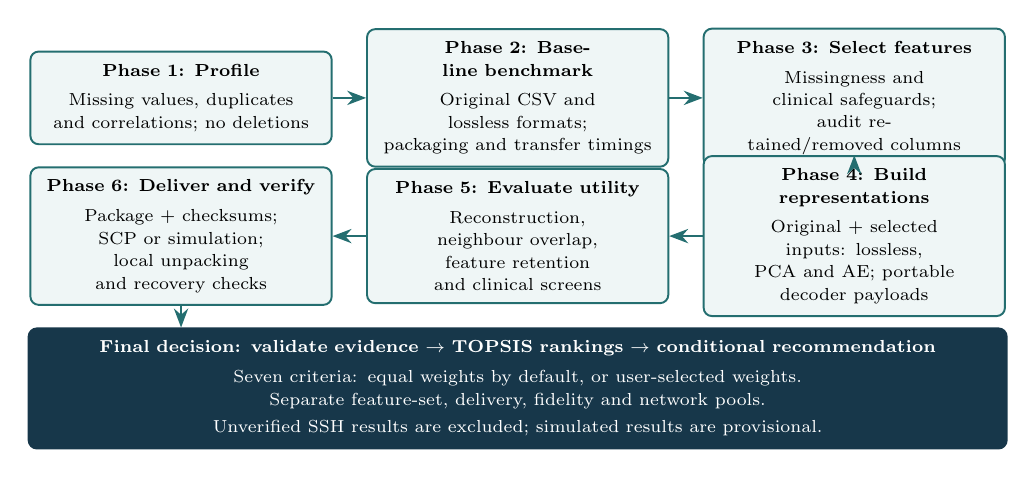
\begin{tikzpicture}[scale=0.9,transform shape,
    phase/.style={draw=accent,fill=pale,rounded corners=3pt,
      line width=0.7pt,text width=3.9cm,minimum height=1.22cm,
      align=center,inner sep=5pt,font=\fontsize{7.5}{9}\selectfont},
    flow/.style={-{Stealth[length=2.4mm]},draw=accent,line width=1pt},
    decision/.style={phase,text width=13.45cm,minimum height=1.25cm,
      fill=ink,text=white,draw=ink}
  ]
    % Top row: left to right.
    \phasebox{p1}{0}{0}{Phase 1: Profile}{Missing values, duplicates\\and correlations; no deletions}
    \phasebox{p2}{4.75}{0}{Phase 2: Baseline benchmark}{Original CSV and lossless formats;\\packaging and transfer timings}
    \phasebox{p3}{9.5}{0}{Phase 3: Select features}{Missingness and clinical safeguards;\\audit retained/removed columns}

    % Second row: right to left. Original and selected inputs enter Phase 4.
    \phasebox{p4}{9.5}{-1.95}{Phase 4: Build representations}{Original + selected inputs: lossless,\\PCA and AE; portable decoder payloads}
    \phasebox{p5}{4.75}{-1.95}{Phase 5: Evaluate utility}{Reconstruction, neighbour overlap,\\feature retention and clinical screens}
    \phasebox{p6}{0}{-1.95}{Phase 6: Deliver and verify}{Package + checksums; SCP or simulation;\\local unpacking and recovery checks}

    \draw[flow] (p1) -- (p2);
    \draw[flow] (p2) -- (p3);
    \draw[flow] (p3) -- (p4);
    \draw[flow] (p4) -- (p5);
    \draw[flow] (p5) -- (p6);

    \node[decision] (final) at (4.75,-4.1) {
      \textbf{Final decision: validate evidence \(\rightarrow\) TOPSIS rankings \(\rightarrow\) conditional recommendation}\\[3pt]
      Seven criteria: equal weights by default, or user-selected weights.
      Separate feature-set, delivery, fidelity and network pools.\\[2pt]
      Unverified SSH results are excluded; simulated results are provisional.
    };
    \draw[flow] (p6.south) -- (p6.south |- final.north);
  \end{tikzpicture}
  \vspace{0.12cm}
  \begin{minipage}{0.97\textwidth}
    \scriptsize
    \textbf{Delivery:} \(T_{\mathrm{package}}+T_{\mathrm{transmit}}+T_{\mathrm{verify}}+
      T_{\mathrm{unpack}}+T_{\mathrm{recover}}\).
    Fresh data additionally charges initial preparation; existing payload excludes it.\\[2pt]
    \textbf{Transfer trials (Phases 2 and 6):} first transfer \(\leq10\) s: 10 total;
    otherwise 1. Retries are separate; model training is not repeated for each transfer.
  \end{minipage}
\end{frame}
\end{document}
